\clearpage
%\newpage

\setcounter{figure}{0}
\renewcommand\thefigure{A.\arabic{figure}}    

\setcounter{table}{0}
\renewcommand{\thetable}{A.\arabic{table}}


\begin{center}
\huge
\textbf{Appendix: NOT FOR PUBLICATION}
\normalsize
\end{center}


\section*{Appendix A: Additional Tables and Figures} \label{sec:appa}
\newpage


\makebox[0.1\width][l]{
\resizebox{\textwidth}{!}{
\begin{tabular}{lccc}
\toprule
\cmidrule(lr){2-4}
& \multicolumn{3}{c}{Standardized GPA}
\cmidrule(lr){2-4}
& Pre-Covid & Covid & Post-Covid  \\
& 2018-2019 & 2020-2021 & 2022-2023  \\
\cmidrule(lr){2-2} \cmidrule(lr){3-3} \cmidrule(lr){4-4}
& (1) & (2) & (3)  \\
\bottomrule
&  &  &   \\
Delay School (After SSA)&      -0.001   &      -0.010   &      -0.004   \\
                    &     (0.006)   &     (0.006)   &     (0.006)   \\
Local Linear        &         Yes   &         Yes   &         Yes   \\
                    &               &               &               \\
Observations        &     418,987   &     371,966   &     485,601   \\
Counterfactual mean &       0.043   &       0.020   &       0.031   \\
Bandwidth           &         365   &         365   &         365   \\
 

\bottomrule
\end{tabular}
}
}


\newpage

\makeatletter
\@ifclassloaded{beamer}{%
       \centering
       \resizebox{0.6\textwidth}{!}%
}{%
       \begin{table}[!tbp]\centering\def\sym#1{\ifmmode^{#1}\else\(^{#1}\)\fi}
       \centering
       \caption{Effects of younger sibling delaying school on older sibling standardized exams - 2 - m - a -  - 365}
       \label{tab:rd_summ_2_m_a_365}
       \resizebox{0.95\textwidth}{!}%
}
{
\makeatother
\makebox[0.1\width][l]{
\resizebox{\textwidth}{!}{
\begin{tabular}{lccc}
\toprule
\cmidrule(lr){2-4}
& \multicolumn{3}{c}{Standardized GPA} \\
\cmidrule(lr){2-4}
& Pre-Covid & Covid & Post-Covid  \\
& 2018-2019 & 2020-2021 & 2022-2023  \\
\cmidrule(lr){2-2} \cmidrule(lr){3-3} \cmidrule(lr){4-4}
& (1) & (2) & (3)  \\
\bottomrule
&  &  &   \\
\multirow{2}{*}{\shortstack[l]{Younger sibling born after \\ school-entry cutoff}}&      -0.000   &      -0.008   &       0.001   \\
                    &     (0.008)   &     (0.007)   &     (0.007)   \\
Local Linear        &         Yes   &         Yes   &         Yes   \\
                    &               &               &               \\
Observations        &     268,561   &     288,245   &     357,788   \\
Counterfactual mean &       0.053   &       0.027   &       0.053   \\
Bandwidth           &         365   &         365   &         365   \\
 

\bottomrule
\end{tabular}
}
\@ifclassloaded{beamer}{%
}{%
       \end{table}
}


\makeatletter
\@ifclassloaded{beamer}{%
       \centering
       \resizebox{0.6\textwidth}{!}%
}{%
       \begin{table}[!tbp]\centering\def\sym#1{\ifmmode^{#1}\else\(^{#1}\)\fi}
       \centering
       \caption{TWFE on GPA by baseline resources}
       \label{tab:twfe_ece_survey_1_pair1}
       \resizebox{0.65\textwidth}{!}%
}
{
\makeatother
\begin{tabular}{lccc}
\toprule
\cmidrule(lr){2-4}
& \multicolumn{3}{c}{TWFE} \\
\cmidrule(lr){2-4}
& 1 sibling & 2 siblings & 3 siblings  \\
\cmidrule(lr){2-2} \cmidrule(lr){3-3} \cmidrule(lr){4-4}
& (1) & (2) & (3)\\
\bottomrule
&  &  &  \\
&  &  &   \\
\multicolumn{4}{l}{\textit{Panel A: All studentes}} \\
\hspace{3mm}Mathematics&      -0.046***&      -0.078***&      -0.077** \\
                    &     (0.013)   &     (0.018)   &     (0.035)   \\
 
%&  &  &   \\
\hspace{3mm}Reading &      -0.023*  &      -0.035*  &      -0.072** \\
                    &     (0.013)   &     (0.018)   &     (0.035)   \\
                    &               &               &               \\
\hspace{3mm}Observations&     108,585   &      85,464   &      72,938   \\
 
&  &  &   \\
\multicolumn{4}{l}{\textit{Panel B: Low SES Households (Q1)}} \\
\hspace{3mm}Mathematics&      -0.026   &      -0.029   &      -0.166***\\
                    &     (0.026)   &     (0.033)   &     (0.057)   \\
 
%&  &  &   \\
\hspace{3mm}Reading &       0.001   &      -0.001   &      -0.133** \\
                    &     (0.026)   &     (0.034)   &     (0.058)   \\
                    &               &               &               \\
\hspace{3mm}Observations&      25,600   &      20,717   &      17,069   \\
 
&  &  &   \\
\multicolumn{4}{l}{\textit{Panel C: High SES Households (Q4)}} \\
\hspace{3mm}Mathematics&      -0.069** &       0.013   &       0.034   \\
                    &     (0.034)   &     (0.056)   &     (0.155)   \\
 
%&  &  &   \\
\hspace{3mm}Reading &      -0.026   &      -0.045   &       0.279*  \\
                    &     (0.034)   &     (0.056)   &     (0.153)   \\
                    &               &               &               \\
\hspace{3mm}Observations&      18,418   &      13,891   &      12,219   \\
 
&  &  &   \\
\multicolumn{4}{l}{\textit{Panel D: Households with no PC or Internet}} \\
\hspace{3mm}Mathematics&      -0.057***&      -0.113***&      -0.058   \\
                    &     (0.020)   &     (0.027)   &     (0.051)   \\
 
%&  &  &   \\
\hspace{3mm}Reading &      -0.036*  &      -0.033   &      -0.069   \\
                    &     (0.020)   &     (0.027)   &     (0.051)   \\
                    &               &               &               \\
\hspace{3mm}Observations&      46,281   &      36,305   &      30,041   \\
 
&  &  &   \\
\multicolumn{4}{l}{\textit{Panel E: Households with both PC and Internet}} \\
\hspace{3mm}Mathematics&      -0.013   &       0.015   &       0.307** \\
                    &     (0.034)   &     (0.056)   &     (0.146)   \\
 
%&  &  &   \\
\hspace{3mm}Reading &       0.009   &       0.006   &       0.505***\\
                    &     (0.035)   &     (0.056)   &     (0.147)   \\
                    &               &               &               \\
\hspace{3mm}Observations&      18,086   &      13,736   &      12,097   \\
 

\bottomrule
\end{tabular}
}
\@ifclassloaded{beamer}{%
}{%
       \end{table}
}

\makeatletter
\@ifclassloaded{beamer}{%
       \centering
       \resizebox{0.6\textwidth}{!}%
}{%
       \begin{table}[!tbp]\centering\def\sym#1{\ifmmode^{#1}\else\(^{#1}\)\fi}
       \centering
       \caption{TWFE on GPA by baseline resources}
       \label{tab:twfe_ece_survey_1_pair2}
       \resizebox{0.65\textwidth}{!}%
}
{
\makeatother
\begin{tabular}{lccc}
\toprule
\cmidrule(lr){2-4}
& \multicolumn{3}{c}{TWFE} \\
\cmidrule(lr){2-4}
& 1 sibling & 2 siblings & 3 siblings  \\
\cmidrule(lr){2-2} \cmidrule(lr){3-3} \cmidrule(lr){4-4}
& (1) & (2) & (3)\\
\bottomrule
&  &  &  \\
&  &  &   \\
\multicolumn{4}{l}{\textit{Panel A: All studentes}} \\
\hspace{3mm}Mathematics&      -0.024***&      -0.062***&      -0.110***\\
                    &     (0.007)   &     (0.010)   &     (0.019)   \\
 
%&  &  &   \\
\hspace{3mm}Reading &      -0.014** &      -0.064***&      -0.077***\\
                    &     (0.007)   &     (0.010)   &     (0.020)   \\
                    &               &               &               \\
\hspace{3mm}Observations&     341,265   &     272,263   &     236,637   \\
 
&  &  &   \\
\multicolumn{4}{l}{\textit{Panel B: Low SES Households (Q1)}} \\
\hspace{3mm}Mathematics&      -0.014   &      -0.048** &      -0.131***\\
                    &     (0.015)   &     (0.019)   &     (0.031)   \\
 
%&  &  &   \\
\hspace{3mm}Reading &      -0.004   &      -0.050***&      -0.073** \\
                    &     (0.015)   &     (0.019)   &     (0.031)   \\
                    &               &               &               \\
\hspace{3mm}Observations&      73,524   &      61,008   &      51,297   \\
 
&  &  &   \\
\multicolumn{4}{l}{\textit{Panel C: High SES Households (Q4)}} \\
\hspace{3mm}Mathematics&      -0.038** &      -0.041   &      -0.203***\\
                    &     (0.016)   &     (0.028)   &     (0.073)   \\
 
%&  &  &   \\
\hspace{3mm}Reading &      -0.029*  &      -0.047*  &      -0.043   \\
                    &     (0.016)   &     (0.028)   &     (0.074)   \\
                    &               &               &               \\
\hspace{3mm}Observations&      70,576   &      54,091   &      48,686   \\
 
&  &  &   \\
\multicolumn{4}{l}{\textit{Panel D: Households with no PC or Internet}} \\
\hspace{3mm}Mathematics&      -0.027*  &      -0.054** &      -0.084*  \\
                    &     (0.014)   &     (0.021)   &     (0.048)   \\
 
%&  &  &   \\
\hspace{3mm}Reading &      -0.015   &      -0.054***&      -0.057   \\
                    &     (0.014)   &     (0.021)   &     (0.048)   \\
                    &               &               &               \\
\hspace{3mm}Observations&     104,804   &      84,220   &      73,029   \\
 
&  &  &   \\
\multicolumn{4}{l}{\textit{Panel E: Households with both PC and Internet}} \\
\hspace{3mm}Mathematics&      -0.036***&      -0.032*  &      -0.144***\\
                    &     (0.012)   &     (0.019)   &     (0.041)   \\
 
%&  &  &   \\
\hspace{3mm}Reading &      -0.027** &      -0.051***&      -0.064   \\
                    &     (0.013)   &     (0.019)   &     (0.042)   \\
                    &               &               &               \\
\hspace{3mm}Observations&     125,843   &      98,884   &      85,077   \\
 

\bottomrule
\end{tabular}
}
\@ifclassloaded{beamer}{%
}{%
       \end{table}
}

\makeatletter
\@ifclassloaded{beamer}{%
       \centering
       \resizebox{0.6\textwidth}{!}%
}{%
       \begin{table}[!tbp]\centering\def\sym#1{\ifmmode^{#1}\else\(^{#1}\)\fi}
       \centering
       \caption{TWFE on 7th grade GPA by 4th grade baseline resources}
       \label{tab:twfe_gpa_baseline_survey_1_pair3}
       \resizebox{0.65\textwidth}{!}%
}
{
\makeatother
\begin{tabular}{lccc}
\toprule
\cmidrule(lr){2-4}
& \multicolumn{3}{c}{TWFE} \\
\cmidrule(lr){2-4}
& 1 sibling & 2 siblings & 3 siblings  \\
\cmidrule(lr){2-2} \cmidrule(lr){3-3} \cmidrule(lr){4-4}
& (1) & (2) & (3)\\
\bottomrule
&  &  &  \\
&  &  &   \\
\multicolumn{4}{l}{\textit{Panel A: All studentes}} \\
\hspace{3mm}Mathematics&      -0.024***&      -0.070***&      -0.060***\\
                    &     (0.007)   &     (0.010)   &     (0.018)   \\
 
%&  &  &   \\
\hspace{3mm}Reading &      -0.021***&      -0.045***&      -0.033*  \\
                    &     (0.007)   &     (0.010)   &     (0.018)   \\
                    &               &               &               \\
\hspace{3mm}Observations&     365,702   &     292,698   &     254,104   \\
 
&  &  &   \\
\multicolumn{4}{l}{\textit{Panel B: Low SES Households (Q1)}} \\
\hspace{3mm}Mathematics&      -0.000   &      -0.020   &      -0.005   \\
                    &     (0.014)   &     (0.017)   &     (0.028)   \\
 
%&  &  &   \\
\hspace{3mm}Reading &      -0.012   &      -0.006   &       0.004   \\
                    &     (0.014)   &     (0.017)   &     (0.028)   \\
                    &               &               &               \\
\hspace{3mm}Observations&      90,252   &      75,485   &      63,910   \\
 
&  &  &   \\
\multicolumn{4}{l}{\textit{Panel C: High SES Households (Q4)}} \\
\hspace{3mm}Mathematics&      -0.026*  &      -0.091***&      -0.106   \\
                    &     (0.016)   &     (0.027)   &     (0.071)   \\
 
%&  &  &   \\
\hspace{3mm}Reading &      -0.031** &      -0.097***&      -0.066   \\
                    &     (0.016)   &     (0.027)   &     (0.072)   \\
                    &               &               &               \\
\hspace{3mm}Observations&      73,259   &      56,234   &      50,652   \\
 
&  &  &   \\
\multicolumn{4}{l}{\textit{Panel D: Households with no PC or Internet}} \\
\hspace{3mm}Mathematics&      -0.018   &      -0.107***&      -0.084*  \\
                    &     (0.013)   &     (0.020)   &     (0.046)   \\
 
%&  &  &   \\
\hspace{3mm}Reading &      -0.021   &      -0.077***&      -0.107** \\
                    &     (0.013)   &     (0.020)   &     (0.047)   \\
                    &               &               &               \\
\hspace{3mm}Observations&     113,464   &      91,731   &      79,607   \\
 
&  &  &   \\
\multicolumn{4}{l}{\textit{Panel E: Households with both PC and Internet}} \\
\hspace{3mm}Mathematics&      -0.007   &      -0.023   &      -0.003   \\
                    &     (0.012)   &     (0.018)   &     (0.040)   \\
 
%&  &  &   \\
\hspace{3mm}Reading &       0.006   &      -0.030*  &      -0.016   \\
                    &     (0.012)   &     (0.018)   &     (0.040)   \\
                    &               &               &               \\
\hspace{3mm}Observations&     136,957   &     108,035   &      92,888   \\
 

\bottomrule
\end{tabular}
}
\@ifclassloaded{beamer}{%
}{%
       \end{table}
}

\makeatletter
\@ifclassloaded{beamer}{%
       \centering
       \resizebox{0.6\textwidth}{!}%
}{%
       \begin{table}[!tbp]\centering\def\sym#1{\ifmmode^{#1}\else\(^{#1}\)\fi}
       \centering
       \caption{TWFE on GPA by baseline resources}
       \label{tab:twfe_ece_survey_1_pair4}
       \resizebox{0.65\textwidth}{!}%
}
{
\makeatother
\begin{tabular}{lccc}
\toprule
\cmidrule(lr){2-4}
& \multicolumn{3}{c}{TWFE} \\
\cmidrule(lr){2-4}
& 1 sibling & 2 siblings & 3 siblings  \\
\cmidrule(lr){2-2} \cmidrule(lr){3-3} \cmidrule(lr){4-4}
& (1) & (2) & (3)\\
\bottomrule
&  &  &  \\
&  &  &   \\
\multicolumn{4}{l}{\textit{Panel A: All studentes}} \\
\hspace{3mm}Mathematics&      -0.032***&      -0.053***&      -0.074***\\
                    &     (0.006)   &     (0.008)   &     (0.014)   \\
 
%&  &  &   \\
\hspace{3mm}Reading &      -0.018***&      -0.035***&      -0.045***\\
                    &     (0.006)   &     (0.008)   &     (0.014)   \\
                    &               &               &               \\
\hspace{3mm}Observations&     466,128   &     384,809   &     339,142   \\
 
&  &  &   \\
\multicolumn{4}{l}{\textit{Panel B: Low SES Households (Q1)}} \\
\hspace{3mm}Mathematics&      -0.018   &      -0.023   &      -0.044** \\
                    &     (0.012)   &     (0.015)   &     (0.021)   \\
 
%&  &  &   \\
\hspace{3mm}Reading &      -0.002   &      -0.006   &      -0.045** \\
                    &     (0.012)   &     (0.015)   &     (0.022)   \\
                    &               &               &               \\
\hspace{3mm}Observations&     119,170   &     103,085   &      90,231   \\
 
&  &  &   \\
\multicolumn{4}{l}{\textit{Panel C: High SES Households (Q4)}} \\
\hspace{3mm}Mathematics&      -0.039***&      -0.074***&      -0.091*  \\
                    &     (0.013)   &     (0.021)   &     (0.050)   \\
 
%&  &  &   \\
\hspace{3mm}Reading &      -0.026*  &      -0.057***&      -0.027   \\
                    &     (0.013)   &     (0.022)   &     (0.050)   \\
                    &               &               &               \\
\hspace{3mm}Observations&      91,916   &      72,508   &      64,890   \\
 
&  &  &   \\
\multicolumn{4}{l}{\textit{Panel D: Households with no PC or Internet}} \\
\hspace{3mm}Mathematics&      -0.032***&      -0.059***&      -0.063** \\
                    &     (0.009)   &     (0.014)   &     (0.029)   \\
 
%&  &  &   \\
\hspace{3mm}Reading &      -0.021** &      -0.036** &       0.004   \\
                    &     (0.010)   &     (0.014)   &     (0.030)   \\
                    &               &               &               \\
\hspace{3mm}Observations&     186,154   &     149,785   &     133,378   \\
 
&  &  &   \\
\multicolumn{4}{l}{\textit{Panel E: Households with both PC and Internet}} \\
\hspace{3mm}Mathematics&      -0.031***&      -0.042***&      -0.095***\\
                    &     (0.010)   &     (0.013)   &     (0.020)   \\
 
%&  &  &   \\
\hspace{3mm}Reading &      -0.005   &      -0.030** &      -0.066***\\
                    &     (0.011)   &     (0.013)   &     (0.021)   \\
                    &               &               &               \\
\hspace{3mm}Observations&     153,436   &     130,307   &     113,257   \\
 

\bottomrule
\end{tabular}
}
\@ifclassloaded{beamer}{%
}{%
       \end{table}
}


\makeatletter
\@ifclassloaded{beamer}{%
       \centering
       \resizebox{0.6\textwidth}{!}%
}{%
       \begin{table}[!tbp]\centering\def\sym#1{\ifmmode^{#1}\else\(^{#1}\)\fi}
       \centering
       \caption{TWFE on 6th grade GPA by 2nd grade baseline achievement and expectations}
       \label{tab:twfe_gpa_baseline_survey_2_pair1}
       \resizebox{0.65\textwidth}{!}%
}
{
\makeatother
\begin{tabular}{lccc}
\toprule
\cmidrule(lr){2-4}
& \multicolumn{3}{c}{TWFE} \\
\cmidrule(lr){2-4}
& 1 sibling & 2 siblings & 3 siblings  \\
\cmidrule(lr){2-2} \cmidrule(lr){3-3} \cmidrule(lr){4-4}
& (1) & (2) & (3)\\
\bottomrule
&  &  &  \\
&  &  &   \\
\multicolumn{4}{l}{\textit{Panel A: All studentes}} \\
\hspace{3mm}Mathematics&      -0.046***&      -0.078***&      -0.077** \\
                    &     (0.013)   &     (0.018)   &     (0.035)   \\
 
%&  &  &   \\
\hspace{3mm}Reading &      -0.023*  &      -0.035*  &      -0.072** \\
                    &     (0.013)   &     (0.018)   &     (0.035)   \\
                    &               &               &               \\
\hspace{3mm}Observations&     108,585   &      85,464   &      72,938   \\
 
&  &  &   \\
\multicolumn{4}{l}{\textit{Panel B: Student in bottom quartile of achievement}} \\
\hspace{3mm}Mathematics&      -0.028   &      -0.073*  &      -0.160** \\
                    &     (0.032)   &     (0.041)   &     (0.072)   \\
 
%&  &  &   \\
\hspace{3mm}Reading &       0.018   &      -0.026   &      -0.095   \\
                    &     (0.032)   &     (0.042)   &     (0.073)   \\
                    &               &               &               \\
\hspace{3mm}Observations&      14,632   &      11,987   &      10,145   \\
 
&  &  &   \\
\multicolumn{4}{l}{\textit{Panel C: Student in top quartile of achievement}} \\
\hspace{3mm}Mathematics&      -0.061** &      -0.103***&       0.030   \\
                    &     (0.026)   &     (0.038)   &     (0.083)   \\
 
%&  &  &   \\
\hspace{3mm}Reading &      -0.049*  &      -0.044   &       0.009   \\
                    &     (0.026)   &     (0.038)   &     (0.084)   \\
                    &               &               &               \\
\hspace{3mm}Observations&      34,500   &      26,134   &      22,113   \\
 
&  &  &   \\
\multicolumn{4}{l}{\textit{Panel D: Max Expectation: Finish school}} \\
\hspace{3mm}Mathematics&       0.004   &      -0.078   &      -0.222   \\
                    &     (0.063)   &     (0.083)   &     (0.141)   \\
 
%&  &  &   \\
\hspace{3mm}Reading &       0.037   &       0.004   &      -0.250*  \\
                    &     (0.064)   &     (0.085)   &     (0.145)   \\
                    &               &               &               \\
\hspace{3mm}Observations&       5,127   &       4,075   &       3,422   \\
 
&  &  &   \\
\multicolumn{4}{l}{\textit{Panel E: Max Expectation: 4-year college or grad school}} \\
\hspace{3mm}Mathematics&      -0.048***&      -0.073***&      -0.041   \\
                    &     (0.015)   &     (0.021)   &     (0.042)   \\
 
%&  &  &   \\
\hspace{3mm}Reading &      -0.030** &      -0.031   &      -0.041   \\
                    &     (0.015)   &     (0.021)   &     (0.043)   \\
                    &               &               &               \\
\hspace{3mm}Observations&      87,535   &      67,871   &      57,831   \\
 

\bottomrule
\end{tabular}
}
\@ifclassloaded{beamer}{%
}{%
       \end{table}
}

\makeatletter
\@ifclassloaded{beamer}{%
       \centering
       \resizebox{0.6\textwidth}{!}%
}{%
       \begin{table}[!tbp]\centering\def\sym#1{\ifmmode^{#1}\else\(^{#1}\)\fi}
       \centering
       \caption{TWFE on 6th grade GPA by 4th grade baseline achievement and expectations}
       \label{tab:twfe_gpa_baseline_survey_2_pair2}
       \resizebox{0.65\textwidth}{!}%
}
{
\makeatother
\begin{tabular}{lccc}
\toprule
\cmidrule(lr){2-4}
& \multicolumn{3}{c}{TWFE} \\
\cmidrule(lr){2-4}
& 1 sibling & 2 siblings & 3 siblings  \\
\cmidrule(lr){2-2} \cmidrule(lr){3-3} \cmidrule(lr){4-4}
& (1) & (2) & (3)\\
\bottomrule
&  &  &  \\
&  &  &   \\
\multicolumn{4}{l}{\textit{Panel A: All studentes}} \\
\hspace{3mm}Mathematics&      -0.024***&      -0.062***&      -0.110***\\
                    &     (0.007)   &     (0.010)   &     (0.019)   \\
 
%&  &  &   \\
\hspace{3mm}Reading &      -0.014** &      -0.064***&      -0.077***\\
                    &     (0.007)   &     (0.010)   &     (0.020)   \\
                    &               &               &               \\
\hspace{3mm}Observations&     341,265   &     272,263   &     236,637   \\
 
&  &  &   \\
\multicolumn{4}{l}{\textit{Panel B: Student in bottom quartile of achievement}} \\
\hspace{3mm}Mathematics&      -0.013   &      -0.052***&      -0.084** \\
                    &     (0.015)   &     (0.020)   &     (0.035)   \\
 
%&  &  &   \\
\hspace{3mm}Reading &      -0.005   &      -0.049** &      -0.078** \\
                    &     (0.015)   &     (0.020)   &     (0.035)   \\
                    &               &               &               \\
\hspace{3mm}Observations&      64,124   &      52,974   &      45,942   \\
 
&  &  &   \\
\multicolumn{4}{l}{\textit{Panel C: Student in top quartile of achievement}} \\
\hspace{3mm}Mathematics&      -0.038** &      -0.094***&      -0.098** \\
                    &     (0.015)   &     (0.022)   &     (0.048)   \\
 
%&  &  &   \\
\hspace{3mm}Reading &      -0.022   &      -0.071***&      -0.095*  \\
                    &     (0.015)   &     (0.023)   &     (0.049)   \\
                    &               &               &               \\
\hspace{3mm}Observations&      97,944   &      74,571   &      64,319   \\
 
&  &  &   \\
\multicolumn{4}{l}{\textit{Panel D: Max Expectation: Finish school}} \\
\hspace{3mm}Mathematics&      -0.021   &      -0.064*  &       0.062   \\
                    &     (0.030)   &     (0.039)   &     (0.065)   \\
 
%&  &  &   \\
\hspace{3mm}Reading &      -0.004   &      -0.082** &      -0.018   \\
                    &     (0.030)   &     (0.039)   &     (0.065)   \\
                    &               &               &               \\
\hspace{3mm}Observations&      22,087   &      18,509   &      15,822   \\
 
&  &  &   \\
\multicolumn{4}{l}{\textit{Panel E: Max Expectation: 4-year college or grad school}} \\
\hspace{3mm}Mathematics&      -0.028***&      -0.061***&      -0.136***\\
                    &     (0.008)   &     (0.012)   &     (0.024)   \\
 
%&  &  &   \\
\hspace{3mm}Reading &      -0.018** &      -0.062***&      -0.106***\\
                    &     (0.008)   &     (0.012)   &     (0.024)   \\
                    &               &               &               \\
\hspace{3mm}Observations&     270,591   &     212,753   &     184,893   \\
 

\bottomrule
\end{tabular}
}
\@ifclassloaded{beamer}{%
}{%
       \end{table}
}

\makeatletter
\@ifclassloaded{beamer}{%
       \centering
       \resizebox{0.6\textwidth}{!}%
}{%
       \begin{table}[!tbp]\centering\def\sym#1{\ifmmode^{#1}\else\(^{#1}\)\fi}
       \centering
       \caption{WFE on GPA by baseline achievement and expectations}
       \label{tab:twfe_gpa_baseline_survey_2_pair3}
       \resizebox{0.65\textwidth}{!}%
}
{
\makeatother
\begin{tabular}{lccc}
\toprule
\cmidrule(lr){2-4}
& \multicolumn{3}{c}{TWFE} \\
\cmidrule(lr){2-4}
& 1 sibling & 2 siblings & 3 siblings  \\
\cmidrule(lr){2-2} \cmidrule(lr){3-3} \cmidrule(lr){4-4}
& (1) & (2) & (3)\\
\bottomrule
&  &  &  \\
&  &  &   \\
\multicolumn{4}{l}{\textit{Panel A: All studentes}} \\
\hspace{3mm}Mathematics&      -0.024***&      -0.070***&      -0.060***\\
                    &     (0.007)   &     (0.010)   &     (0.018)   \\
 
%&  &  &   \\
\hspace{3mm}Reading &      -0.021***&      -0.045***&      -0.033*  \\
                    &     (0.007)   &     (0.010)   &     (0.018)   \\
                    &               &               &               \\
\hspace{3mm}Observations&     365,702   &     292,698   &     254,104   \\
 
&  &  &   \\
\multicolumn{4}{l}{\textit{Panel B: Student in bottom quartile of achievement}} \\
\hspace{3mm}Mathematics&       0.022   &      -0.009   &      -0.101***\\
                    &     (0.015)   &     (0.019)   &     (0.033)   \\
 
%&  &  &   \\
\hspace{3mm}Reading &       0.020   &      -0.005   &      -0.015   \\
                    &     (0.015)   &     (0.020)   &     (0.034)   \\
                    &               &               &               \\
\hspace{3mm}Observations&      76,396   &      63,590   &      55,311   \\
 
&  &  &   \\
\multicolumn{4}{l}{\textit{Panel C: Student in top quartile of achievement}} \\
\hspace{3mm}Mathematics&      -0.046***&      -0.118***&      -0.166***\\
                    &     (0.014)   &     (0.021)   &     (0.045)   \\
 
%&  &  &   \\
\hspace{3mm}Reading &      -0.042***&      -0.081***&      -0.062   \\
                    &     (0.014)   &     (0.021)   &     (0.045)   \\
                    &               &               &               \\
\hspace{3mm}Observations&     100,921   &      76,928   &      66,386   \\
 
&  &  &   \\
\multicolumn{4}{l}{\textit{Panel D: Max Expectation: Finish school}} \\
\hspace{3mm}Mathematics&       0.018   &      -0.033   &      -0.035   \\
                    &     (0.029)   &     (0.037)   &     (0.060)   \\
 
%&  &  &   \\
\hspace{3mm}Reading &      -0.085***&      -0.057   &      -0.051   \\
                    &     (0.029)   &     (0.037)   &     (0.060)   \\
                    &               &               &               \\
\hspace{3mm}Observations&      26,308   &      22,144   &      19,072   \\
 
&  &  &   \\
\multicolumn{4}{l}{\textit{Panel E: Max Expectation: 4-year college or grad school}} \\
\hspace{3mm}Mathematics&      -0.032***&      -0.087***&      -0.092***\\
                    &     (0.008)   &     (0.011)   &     (0.022)   \\
 
%&  &  &   \\
\hspace{3mm}Reading &      -0.024***&      -0.057***&      -0.076***\\
                    &     (0.008)   &     (0.011)   &     (0.023)   \\
                    &               &               &               \\
\hspace{3mm}Observations&     287,508   &     226,685   &     196,682   \\
 

\bottomrule
\end{tabular}
}
\@ifclassloaded{beamer}{%
}{%
       \end{table}
}

\makeatletter
\@ifclassloaded{beamer}{%
       \centering
       \resizebox{0.6\textwidth}{!}%
}{%
       \begin{table}[!tbp]\centering\def\sym#1{\ifmmode^{#1}\else\(^{#1}\)\fi}
       \centering
       \caption{TWFE on 9th grade GPA by 8th grade baseline achievement and expectations}
       \label{tab:twfe_gpa_baseline_survey_2_pair4}
       \resizebox{0.65\textwidth}{!}%
}
{
\makeatother
\begin{tabular}{lccc}
\toprule
\cmidrule(lr){2-4}
& \multicolumn{3}{c}{TWFE} \\
\cmidrule(lr){2-4}
& 1 sibling & 2 siblings & 3 siblings  \\
\cmidrule(lr){2-2} \cmidrule(lr){3-3} \cmidrule(lr){4-4}
& (1) & (2) & (3)\\
\bottomrule
&  &  &  \\
&  &  &   \\
\multicolumn{4}{l}{\textit{Panel A: All studentes}} \\
\hspace{3mm}Mathematics&      -0.032***&      -0.053***&      -0.074***\\
                    &     (0.006)   &     (0.008)   &     (0.014)   \\
 
%&  &  &   \\
\hspace{3mm}Reading &      -0.018***&      -0.035***&      -0.045***\\
                    &     (0.006)   &     (0.008)   &     (0.014)   \\
                    &               &               &               \\
\hspace{3mm}Observations&     466,128   &     384,809   &     339,142   \\
 
&  &  &   \\
\multicolumn{4}{l}{\textit{Panel B: Student in bottom quartile of achievement}} \\
\hspace{3mm}Mathematics&       0.001   &      -0.043***&      -0.104***\\
                    &     (0.012)   &     (0.015)   &     (0.023)   \\
 
%&  &  &   \\
\hspace{3mm}Reading &       0.012   &      -0.049***&      -0.079***\\
                    &     (0.012)   &     (0.016)   &     (0.024)   \\
                    &               &               &               \\
\hspace{3mm}Observations&     100,937   &      86,703   &      76,726   \\
 
&  &  &   \\
\multicolumn{4}{l}{\textit{Panel C: Student in top quartile of achievement}} \\
\hspace{3mm}Mathematics&      -0.062***&      -0.100***&      -0.171***\\
                    &     (0.012)   &     (0.018)   &     (0.037)   \\
 
%&  &  &   \\
\hspace{3mm}Reading &      -0.030** &      -0.065***&      -0.091** \\
                    &     (0.012)   &     (0.018)   &     (0.037)   \\
                    &               &               &               \\
\hspace{3mm}Observations&     127,522   &     100,695   &      88,372   \\
 
&  &  &   \\
\multicolumn{4}{l}{\textit{Panel D: Max Expectation: Finish school}} \\
\hspace{3mm}Mathematics&       0.028   &       0.033   &      -0.071   \\
                    &     (0.025)   &     (0.032)   &     (0.052)   \\
 
%&  &  &   \\
\hspace{3mm}Reading &       0.017   &       0.060*  &      -0.031   \\
                    &     (0.026)   &     (0.034)   &     (0.056)   \\
                    &               &               &               \\
\hspace{3mm}Observations&      25,985   &      21,700   &      18,777   \\
 
&  &  &   \\
\multicolumn{4}{l}{\textit{Panel E: Max Expectation: 4-year college or grad school}} \\
\hspace{3mm}Mathematics&      -0.036***&      -0.061***&      -0.084***\\
                    &     (0.007)   &     (0.009)   &     (0.016)   \\
 
%&  &  &   \\
\hspace{3mm}Reading &      -0.019***&      -0.043***&      -0.059***\\
                    &     (0.007)   &     (0.009)   &     (0.016)   \\
                    &               &               &               \\
\hspace{3mm}Observations&     389,469   &     319,269   &     281,150   \\
 

\bottomrule
\end{tabular}
}
\@ifclassloaded{beamer}{%
}{%
       \end{table}
}



\begin{figure}[htbp]
         \centering
        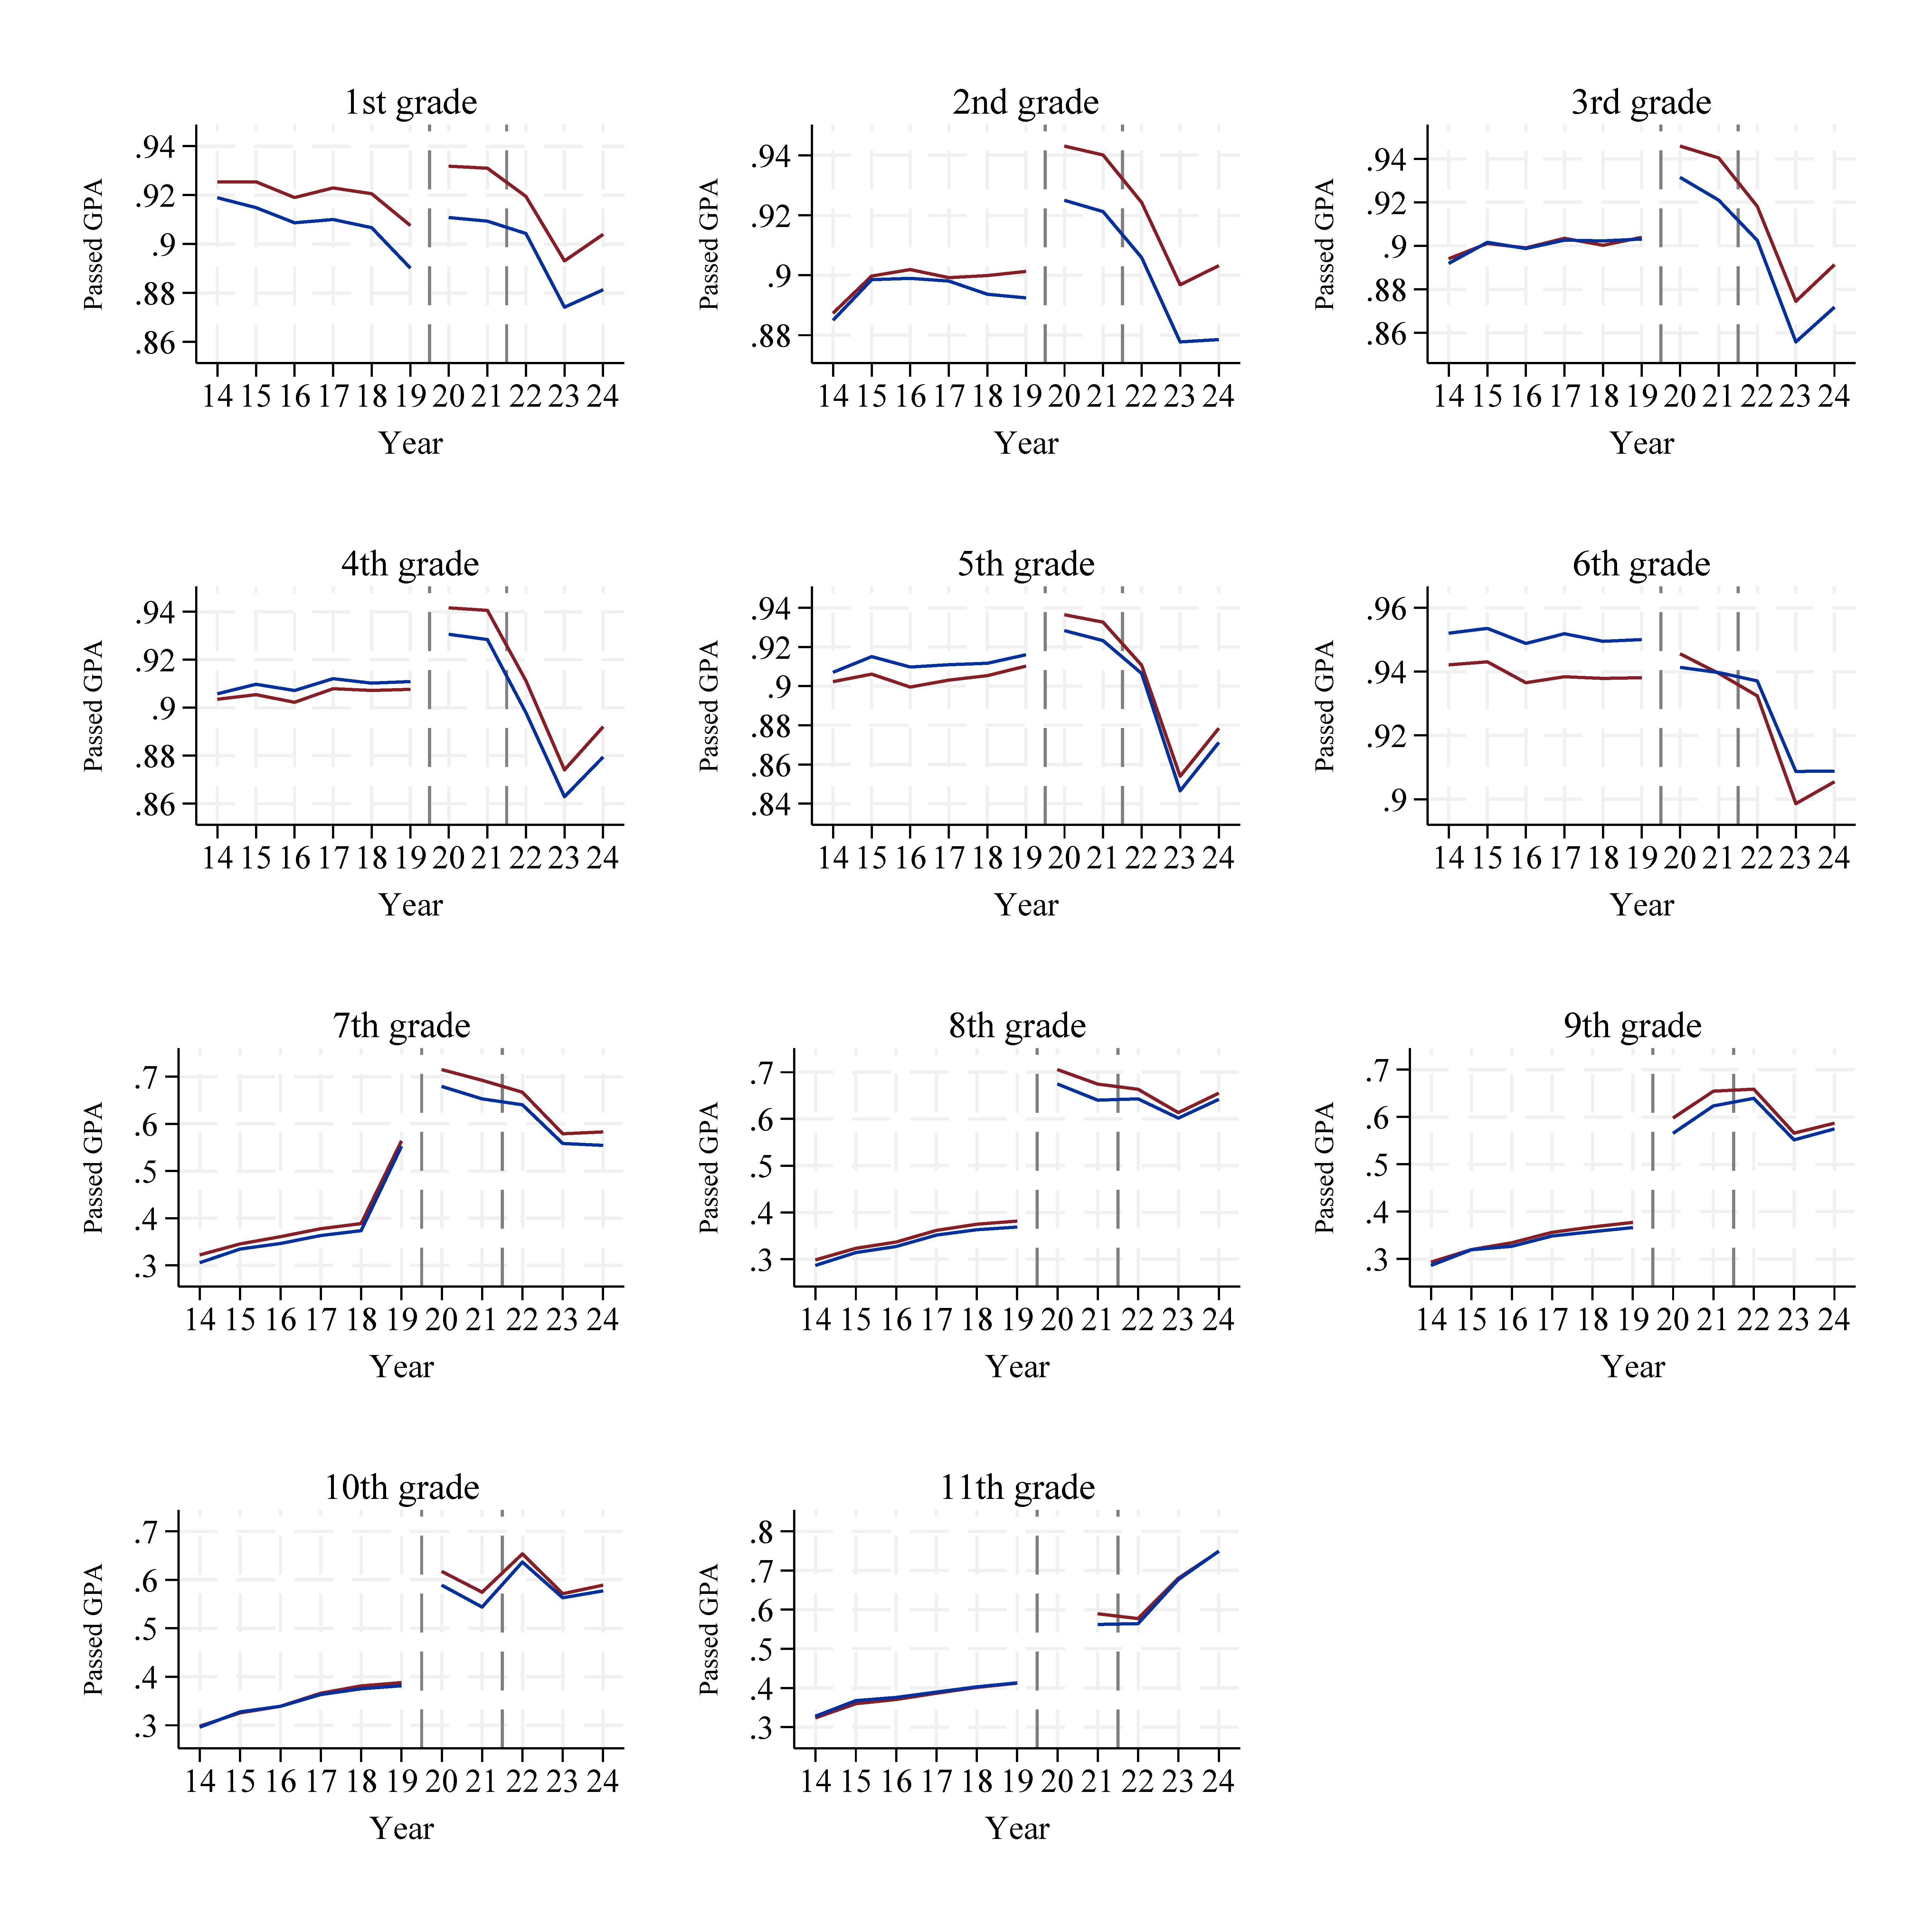
\includegraphics[width=\textwidth]{./FIGURES/Descriptive/raw_grades_pass_math_siblings.pdf}
        \caption{\% of students with an A in Mathematics for each grade 1st-1th}
        \label{fig:trend_pass_grades}
\end{figure}

\begin{figure}[htbp]
         \centering
        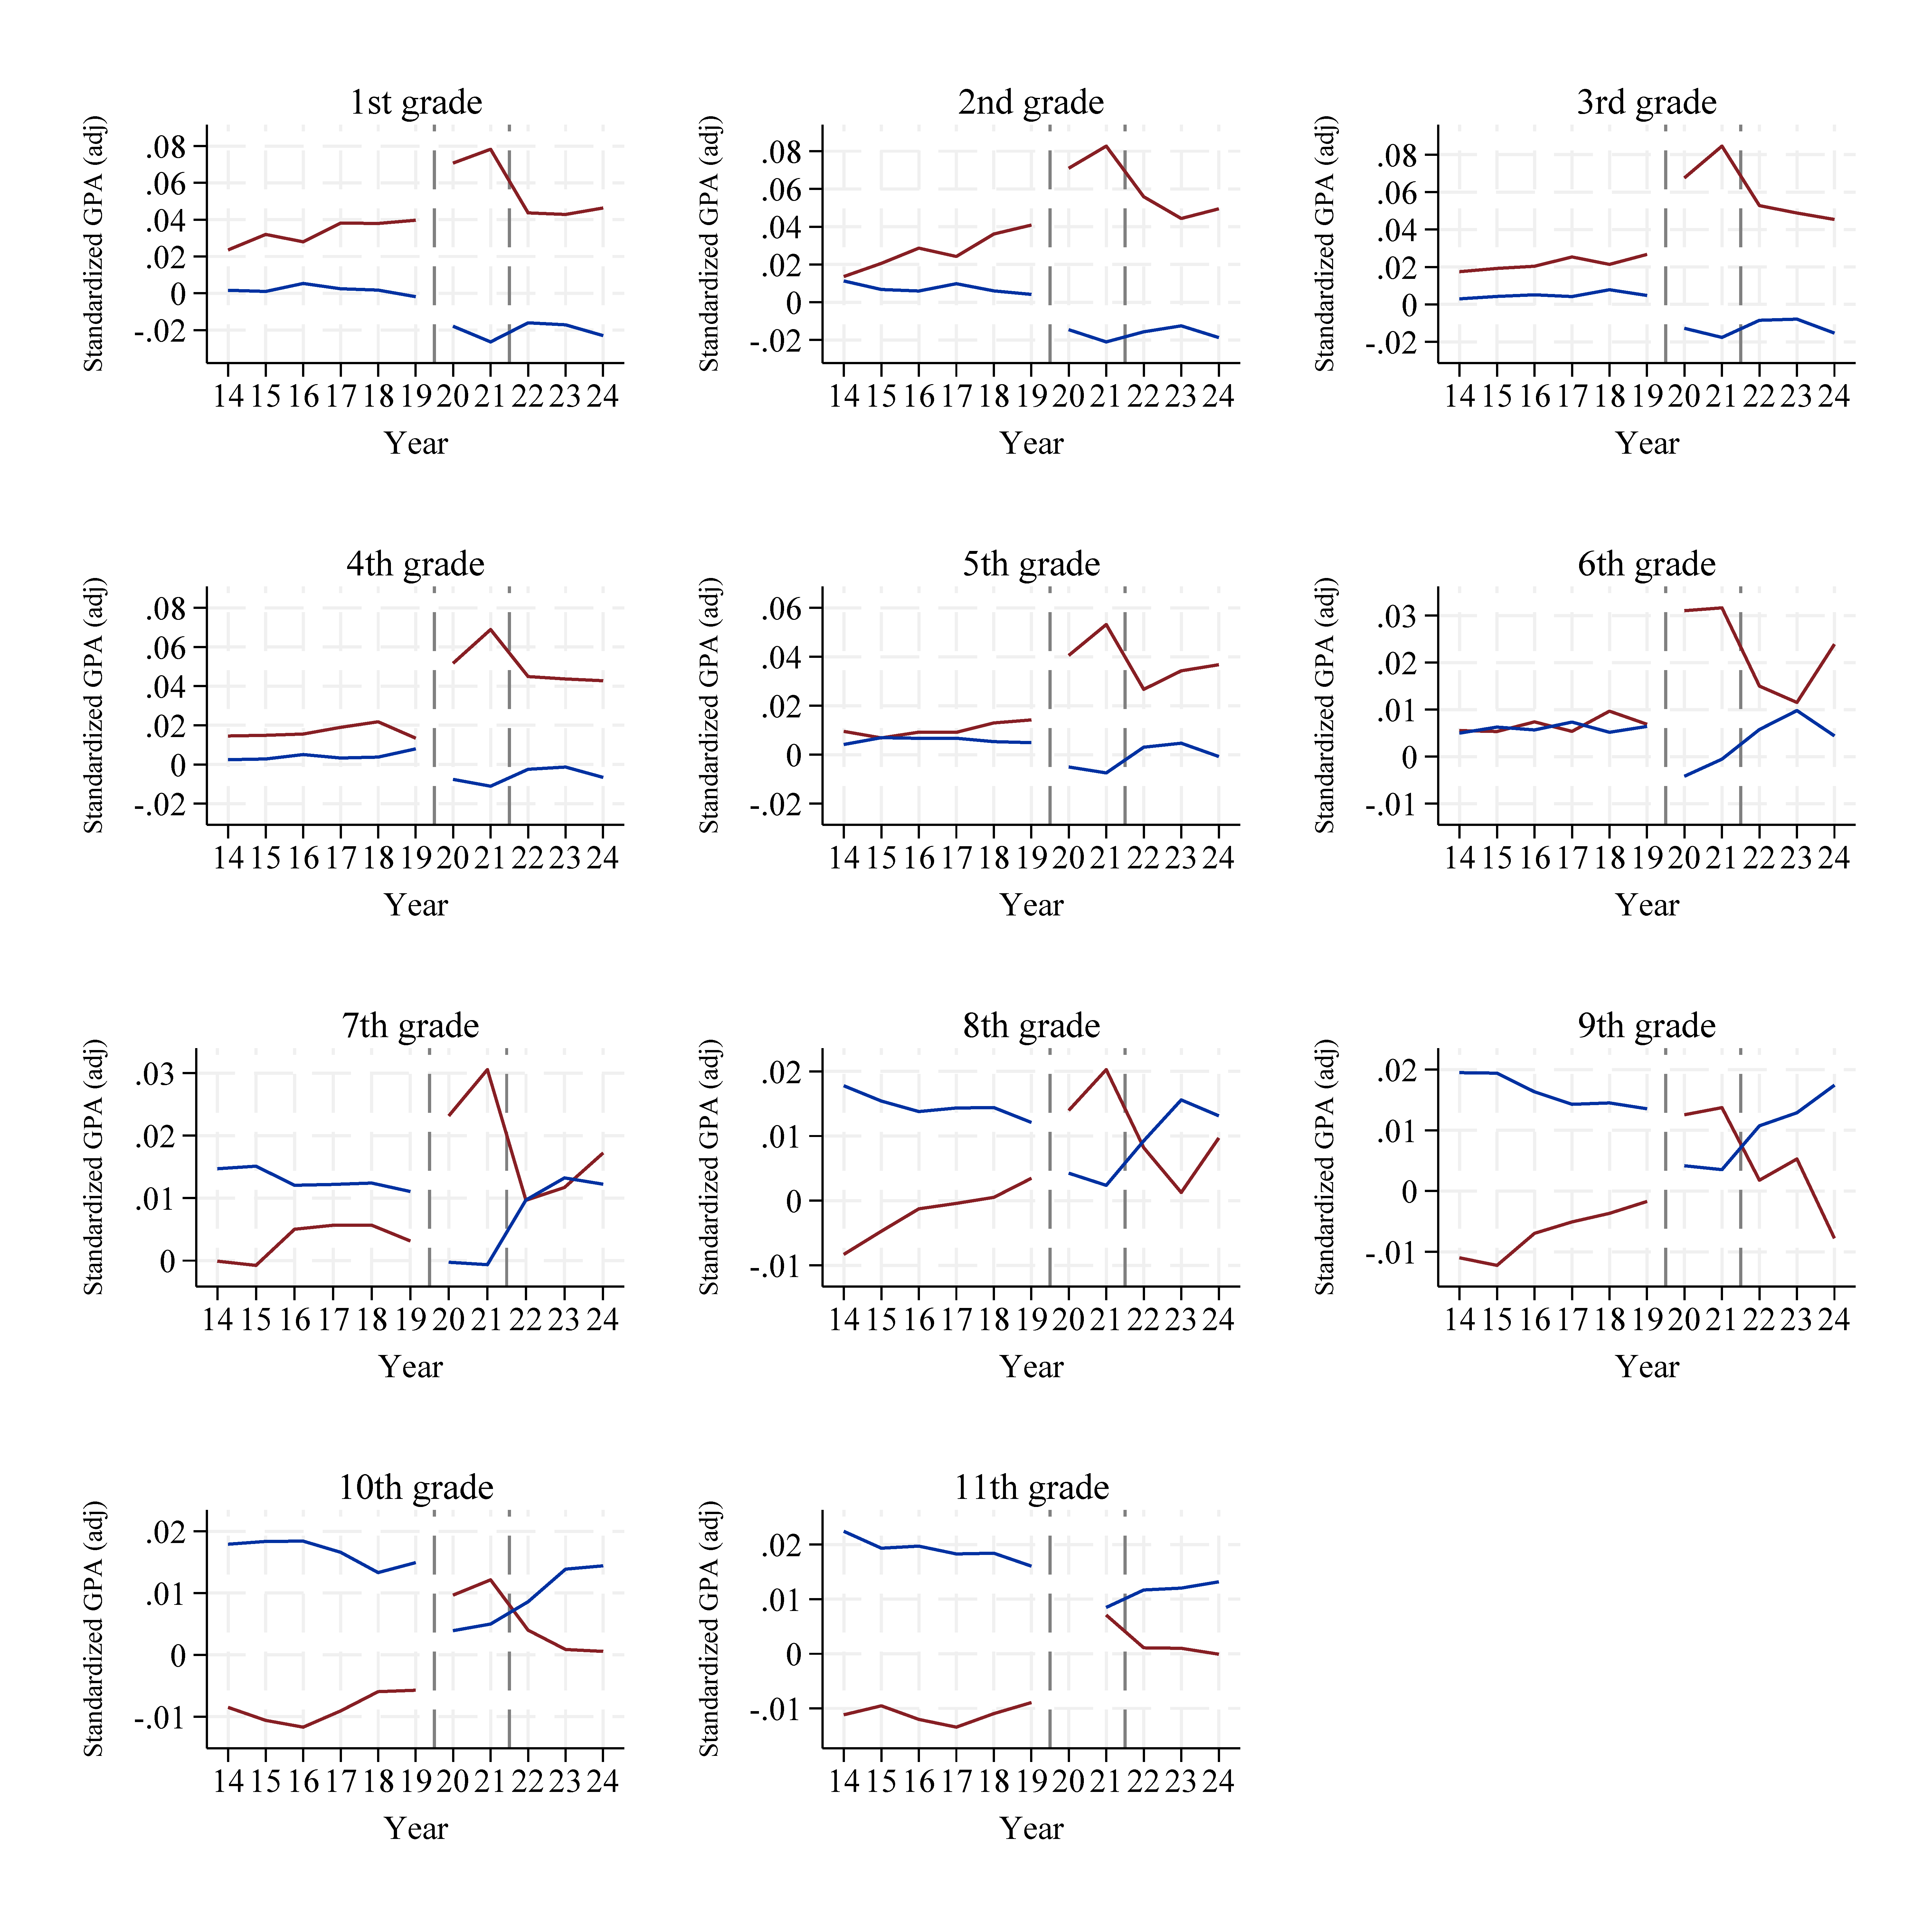
\includegraphics[width=\textwidth]{./FIGURES/Descriptive/raw_grades_std_gpa_m_adj_siblings.pdf}
        \caption{Average GPA standardized within school-grade-year for each grade 1st-1th}
        \label{fig:trend_gpa_grades}
\end{figure}



\begin{figure}[htbp]
    \centering
    
        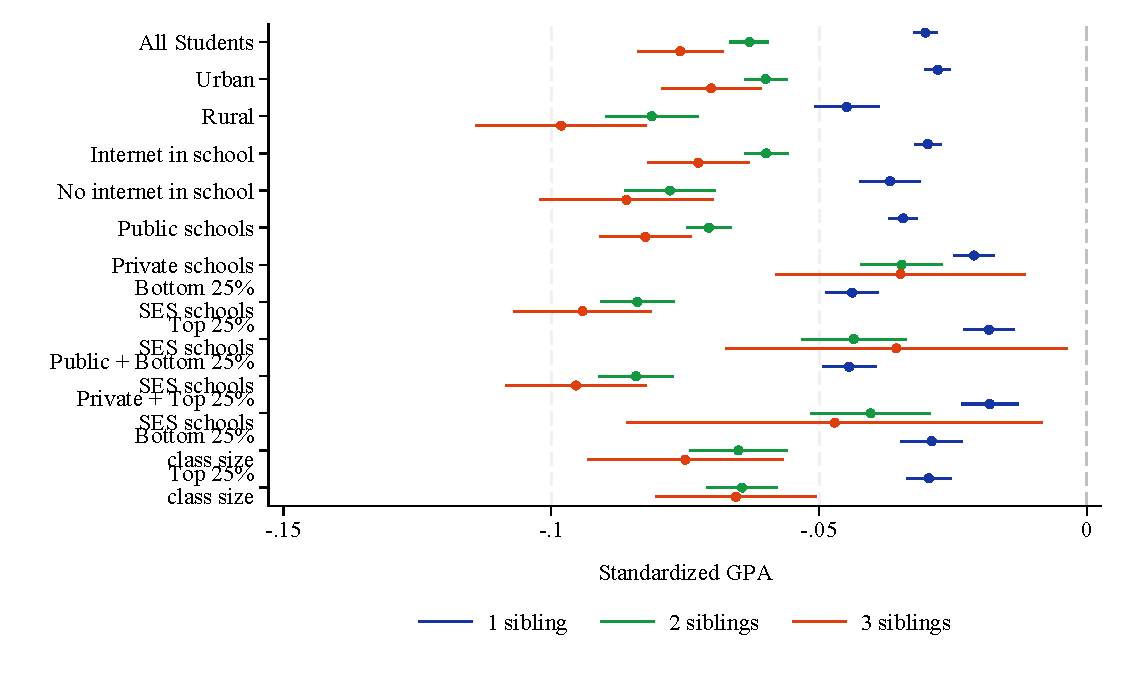
\includegraphics[width=\textwidth]{./FIGURES/TWFE/covid_twfe_A_bysibs_elm_all_gpa_m_adj_Tsiblings_Soldest_4.pdf}
        \caption{Change in gap between children with siblings and only childs}
        \label{fig:fig_appA}

\end{figure}

\begin{figure}[htbp]
    \centering
    
        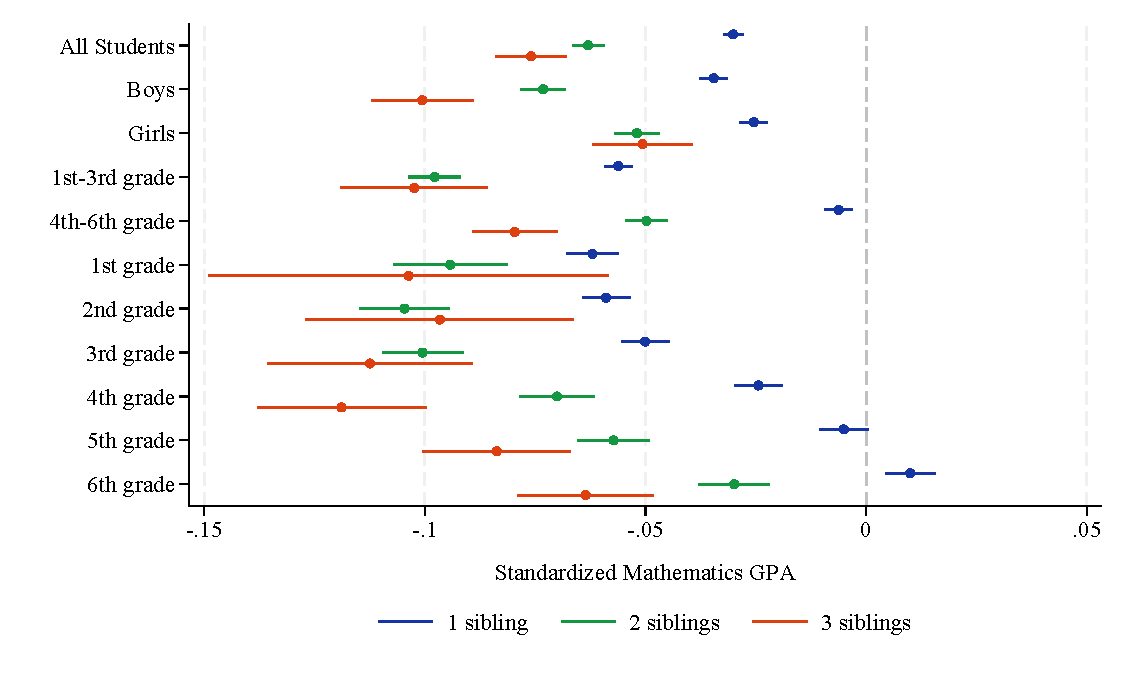
\includegraphics[width=\textwidth]{./FIGURES/TWFE/covid_twfe_B_bysibs_elm_all_gpa_m_adj_Tsiblings_Soldest_4.pdf}
        \caption{Change in gap between children with siblings and only childs}
        \label{fig:fig_appB}

\end{figure}

\begin{figure}[htbp]
    \centering
    
        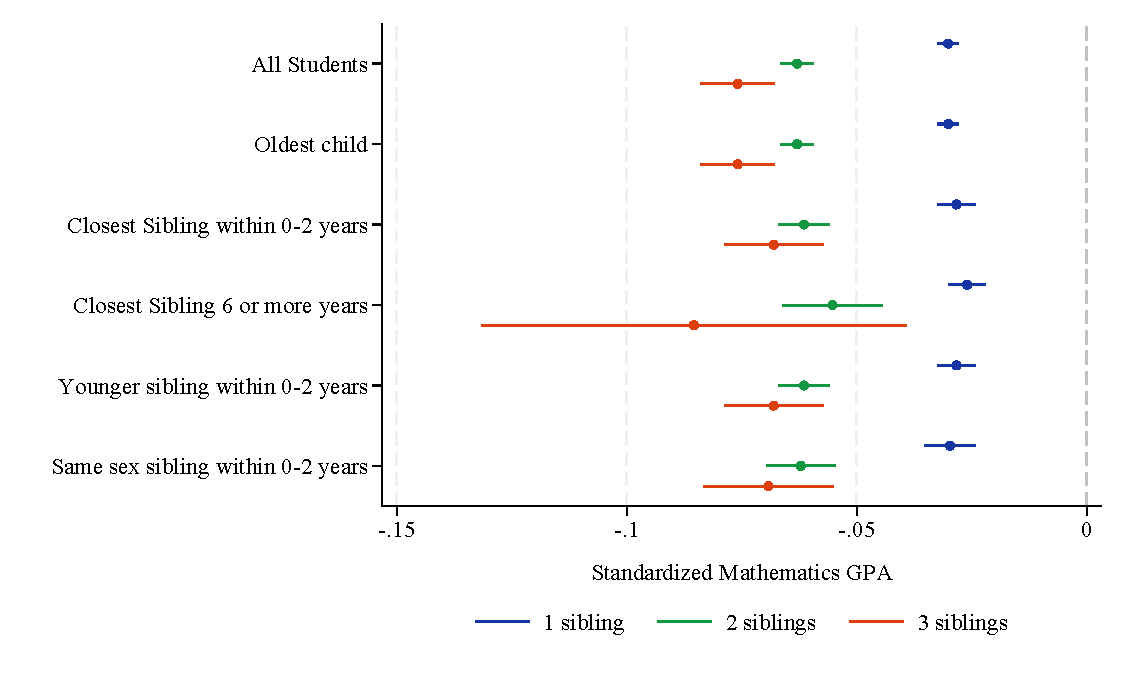
\includegraphics[width=\textwidth]{./FIGURES/TWFE/covid_twfe_C_bysibs_elm_all_gpa_m_adj_Tsiblings_Soldest_4.pdf}
        \caption{Change in gap between children with siblings and only childs}
        \label{fig:fig_appC}

\end{figure}


\begin{figure}[htbp]
    \centering
    
        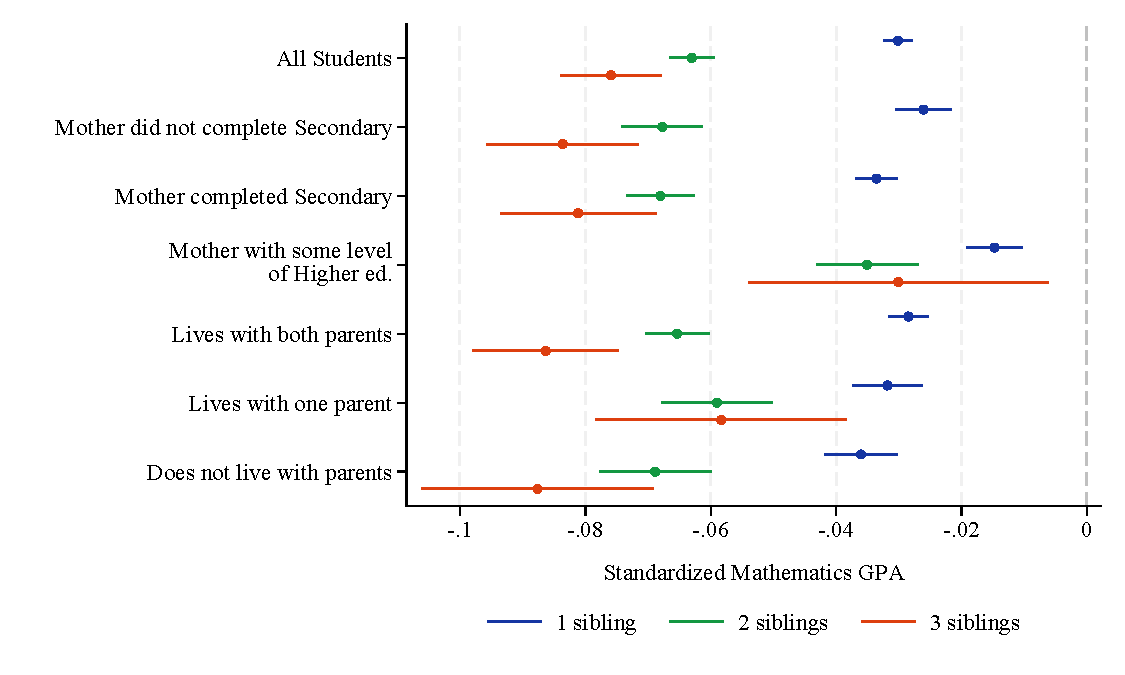
\includegraphics[width=\textwidth]{./FIGURES/TWFE/covid_twfe_D_bysibs_elm_all_gpa_m_adj_Tsiblings_Soldest_4.pdf}
        \caption{Change in gap between children with siblings and only childs}
        \label{fig:fig_appD}

\end{figure}

\clearpage

\section*{Appendix B: Validating Sibling Identification} \label{sec:appB}

\subsection{Contrasting with survey responses}


\subsection{Number of siblings}

In \textcolor{green}{XX} one survey question asked about number of siblings.


\subsection{Number of people in the household}

In the 2nd grade survey in 2015 and 2016 a question asked about the number of adults and children in the household. In \textcolor{green}{XX} I show the distribution of responses by number of children estimated with matching parent IDs. 

\newpage